\chapter{Análisis}

\section{Domain-Driven Design}

En este capítulo, realizaremos un análisis detallado de los requisitos del proyecto utilizando la metodología del Diseño Orientado al Dominio o \textit{domain-driven design} que para mayor rapidez y concisión denominaremos como \textit{DDD}. Esta filosofía de desarrollo de software nos ayudará a comprender y modelar el dominio empresarial, asegurando que nuestras soluciones se alineen con las necesidades específicas de los usuarios y del negocio.

El Diseño Orientado al Dominio (DDD) es una filosofía de desarrollo de software que se centra en comprender y modelar el dominio empresarial para alinear el software con las necesidades del negocio. Introducido por Eric Evans en su libro~\cite{evans2004domain}, DDD ha evolucionado con aportes de numerosos profesionales.

En esencia, \textit{DDD} aborda la complejidad enfocándose en el ``dominio'', el contexto específico del software. Promueve el uso de un ``lenguaje ubicuo'', un lenguaje común entre desarrolladores y partes interesadas, para garantizar que el software refleje con precisión el ámbito empresarial. La modelización en \textit{DDD} no busca crear el modelo más realista, sino uno útil y apropiado para su propósito, similar a cómo una película representa la realidad de manera selectiva para cumplir su objetivo.

Hemos elegido \textit{DDD} porque proporciona una estructura clara y coherente para manejar la complejidad del dominio del proyecto, asegurando que las soluciones técnicas se alineen estrechamente con las necesidades del negocio y los usuarios. Esta metodología nos permitirá identificar y definir las entidades principales que se necesitan para satisfacer los requisitos del sistema, facilitando la comunicación y la comprensión entre todas las partes involucradas.

Hoy en día, DDD sigue siendo ampliamente utilizado en diversos proyectos, con numerosos casos de éxito en la industria que demuestran su eficacia, como se detalla en esta \href{https://blog.bitsrc.io/demystifying-domain-driven-design-ddd-in-modern-software-architecture-b57e27c210f7}{publicación}. Empresas como Netflix, Uber y Airbnb han adoptado DDD con notable éxito.

\subsection{Enfoque Ágil y DDD}

Es importante destacar que el diseño impulsado por el dominio (Domain-Driven Design, DDD) en~\cite{evans2004domain} no abandona la filosofía ágil. Aunque este libro no está vinculado a una metodología en particular, se orienta hacia la nueva familia de ``procesos de desarrollo ágil''. Específicamente, asume que se emplean dos prácticas en el proyecto, las cuales son prerrequisitos para aplicar el enfoque presentado en este libro.

\begin{itemize}
    \item \textbf{El desarrollo es iterativo.}
    \item \textbf{Relación estrecha entre quiénes conocen el dominio y quiénes saben cómo construir \textit{software}.}
\end{itemize}

\section{Análisis de requisitos}

Los requisitos han sido identificados a partir de las historias de usuario \ref{sec:historias_usuario} anteriormente definidas y los usuarios identificados en \ref{sec:usuarios_identificados}. Estos requisitos son los que llamamos los requisitos básicos o esenciales a partir de los cuales se desarrollará el diseño.

\begin{itemize}
    \item \textbf{Se debe proporcionar un editor de memes.}
    \begin{itemize}
        \item[-] Historias de usuario requeridas: HU01, HU04 y HU02.
    \end{itemize}
    \item \textbf{Se debe proporcionar un catálogo de memes predefinidos.}
    \begin{itemize}
        \item[-] Historias de usuario requeridas: HU01, HU02 y HU03.
    \end{itemize}
    \item \textbf{La solución debe poder permitir colaboración en la creación de memes.}
    \begin{itemize}
        \item[-] Historias de usuario requeridas: HU04.
    \end{itemize}
    \item \textbf{Se debe proporcionar un sistema de búsqueda avanzada de memes.}
    \begin{itemize}
        \item[-] Historias de usuario requeridas: HU03.
    \end{itemize} 
\end{itemize}

En cada una de las secciones siguientes se va a ir introduciendo cierta terminología de DDD para ir analizando y entendiendo el modelo en el que el proyecto se mueve. En cada una de ellas, se va a ir explicando a qué se refiere ese término y su aplicación.

\section{Lenguaje ubicuo en DDD}

El lenguaje ubicuo es el término que se utiliza en DDD para referirse a un lenguaje común que se utiliza en todo el proyecto. Este lenguaje compartido por todos es esencial para la comunicación y la comprensión entre todas las partes interesadas. En este debe basarse el modelo del dominio por lo que debe ser riguroso y preciso para evitar cualquier tipo de ambigüedad. De igual manera, debe ser especificado en una etapa temprana del proyecto por eso, está antes de todo el proceso. A continuación, los términos del lenguaje ubicuo:

\begin{itemize}
    \item \textbf{Meme}: imagen, vídeo o texto que difunde un mensaje que suele ser humorístico.
    \item \textbf{Plantilla}: formato base sobre la que se crean los memes.
    \item \textbf{Catálogo de memes}: almacenamiento centralizado de memes.
    \item \textbf{Colaborador}: usuario que puede editar un meme.
    \item \textbf{Visualizador}: usuario que puede ver un meme.
    \item \textbf{Búsqueda avanzada}: sistema de búsqueda en el catálogo de memes que permite filtrar memes por diferentes criterios.
\end{itemize}

\section{\textit{Core domain}}

En DDD, este es el corazón de cualquier proyecto que impulsa lo que hace y define si es un éxito o en su defecto, es un fracaso. En nuestro caso, el \textit{core domain} es la \textbf{gestión centralizada y colaborativa de memes}. Este dominio englobará todas las capacidades que el sistema permita a los usuarios realizar con los memes, como la creación, edición, búsqueda, colaboración, etc.

Este dominio requiere un profundo conocimiento del campo en cuestión por lo que la mejor forma de abordarlo es mediante el \textit{event storming}. Esta es una manera de explorar rápidamente los dominios centrándose en los eventos de dominio que son algo que ha ocurrido en el dominio y son relevantes. Esta técnica fue introducida y popularizada por Alberto Brandolini en~\cite{brandolini2013introducing} aunque este ejemplo está basado en este artículo de \href{https://ibm-cloud-architecture.github.io/refarch-eda/methodology/event-storming/}{IBM Automation - Sharing knowledge}.

Para realizar un primer diagrama de eventos vamos a definir un conjunto inicial de conceptos y su formato con el que se van a utilizar:

\begin{itemize}
    \item Eventos de dominio: notas de color naranja y verbos en pasado.
    \item Comentarios o preguntas notas de color rojo indicando puntos peligrosos, importantes y que se debe hacer más hincapié.
    \item Definiciones de conceptos: notas de color gris para ayudar a entender el contexto y lenguaje ubicuo.
    \item Actores: notas de color amarillo.
    \item Comandos: notas de color azul y verbos en infinitivo que indican acción, intención o decisión.
    \item Entidades del dominio: notas de color verde. Estas son necesarias para aportar información que se necesita para apoyar la realización de los eventos.
    \item Políticas: notas de color rosa. Empiezan siempre con \textit{siempre que} y representan reglas que se deben cumplir antes de que el evento ocurra o puede hacer que estos se ejecuten.
\end{itemize}

\begin{figure}[ht]
    \caption{Formato de conceptos.}
    \centering
    \vspace*{0.5cm}
    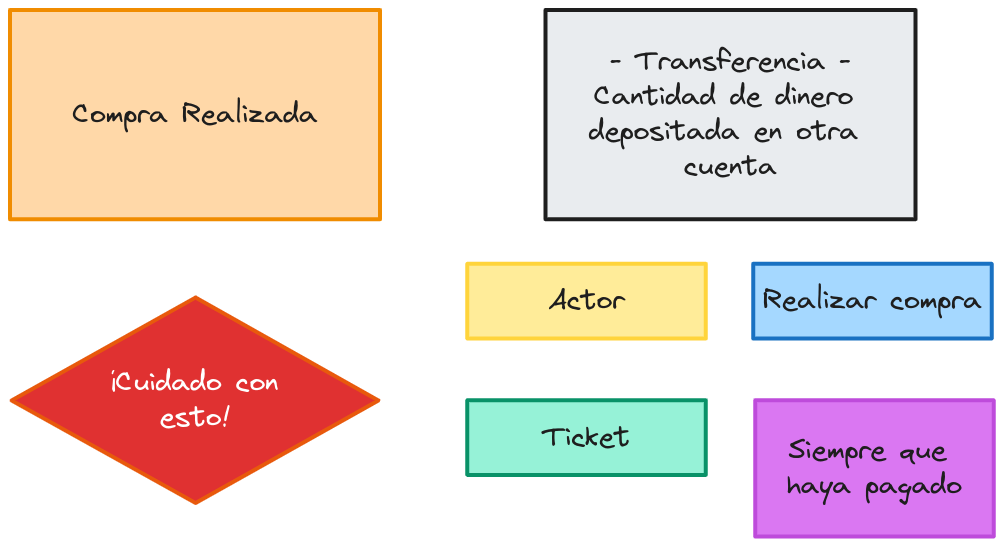
\includegraphics[scale=0.25]{figuras/conceptos.png}
\end{figure}

El siguiente paso tras definir el formato de las notas es identificar todos los eventos relevantes en el dominio, escribir una descripción corta de cada uno de ellos y colocarlos en la secuencia de tiempo. Para ayudar al entendimiento se necesita saber quién ha iniciado el evento y qué información ha permitido que ocurra.

\subsection{Descubrimiento de eventos de dominio}

En esta etapa simplemente se describe qué ha pasado en el dominio. No se debe preocupar por cómo se va a implementar, simplemente se debe describir lo que ha ocurrido.

\begin{figure}[ht]
    \caption{Eventos de dominio.}
    \centering
    \vspace*{0.5cm}
    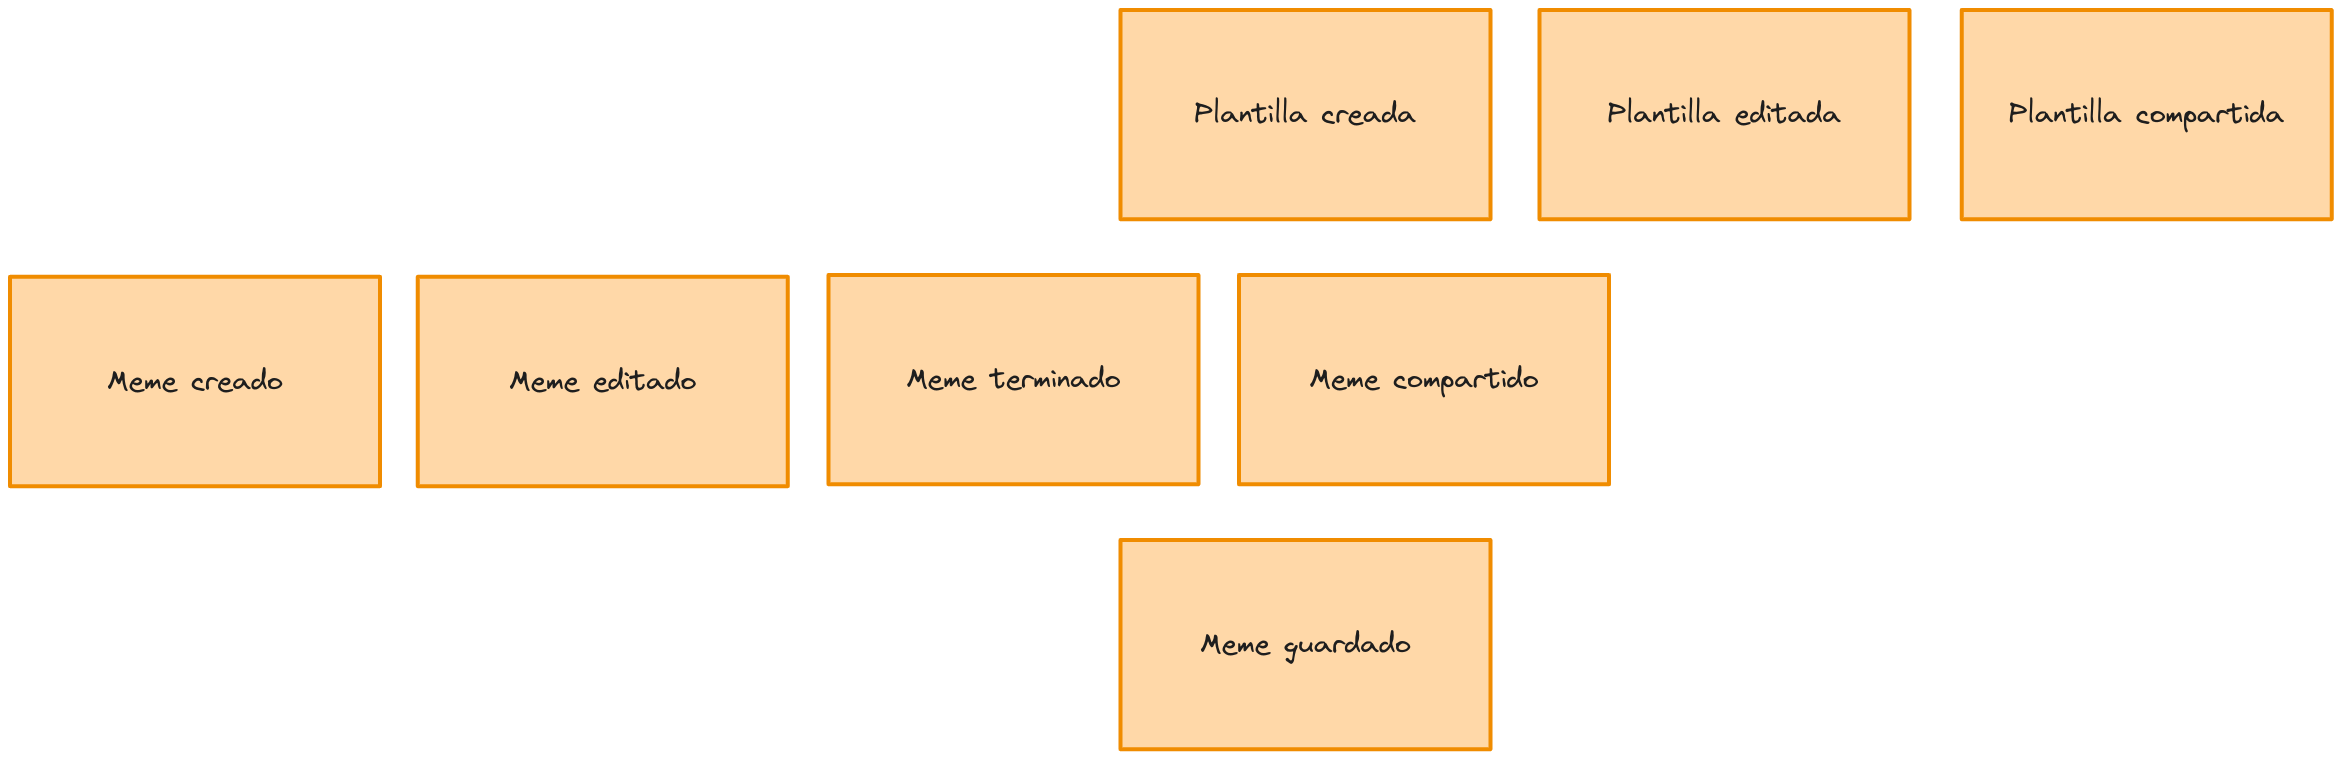
\includegraphics[scale=0.15]{figuras/eventosdominio.png}
\end{figure}

Por ahora, no hay que preocuparse si algunos eventos se sobreponen.

\subsection{¡Cuenta la historia!}

En este paso, se debería contar qué está ocurriendo en el diagrama y colocar sobre el mismo las preguntas y dudas que puedan surgir. Aquí se hace una especie de reflexión y refinamiento. Por lo tanto, vamos a colocar en el diagrama las notas rojas para indicar los puntos que se deben aclarar.

\begin{figure}[ht]
    \caption{Eventos de dominio con puntos de reflexión.}
    \centering
    \vspace*{0.5cm}
    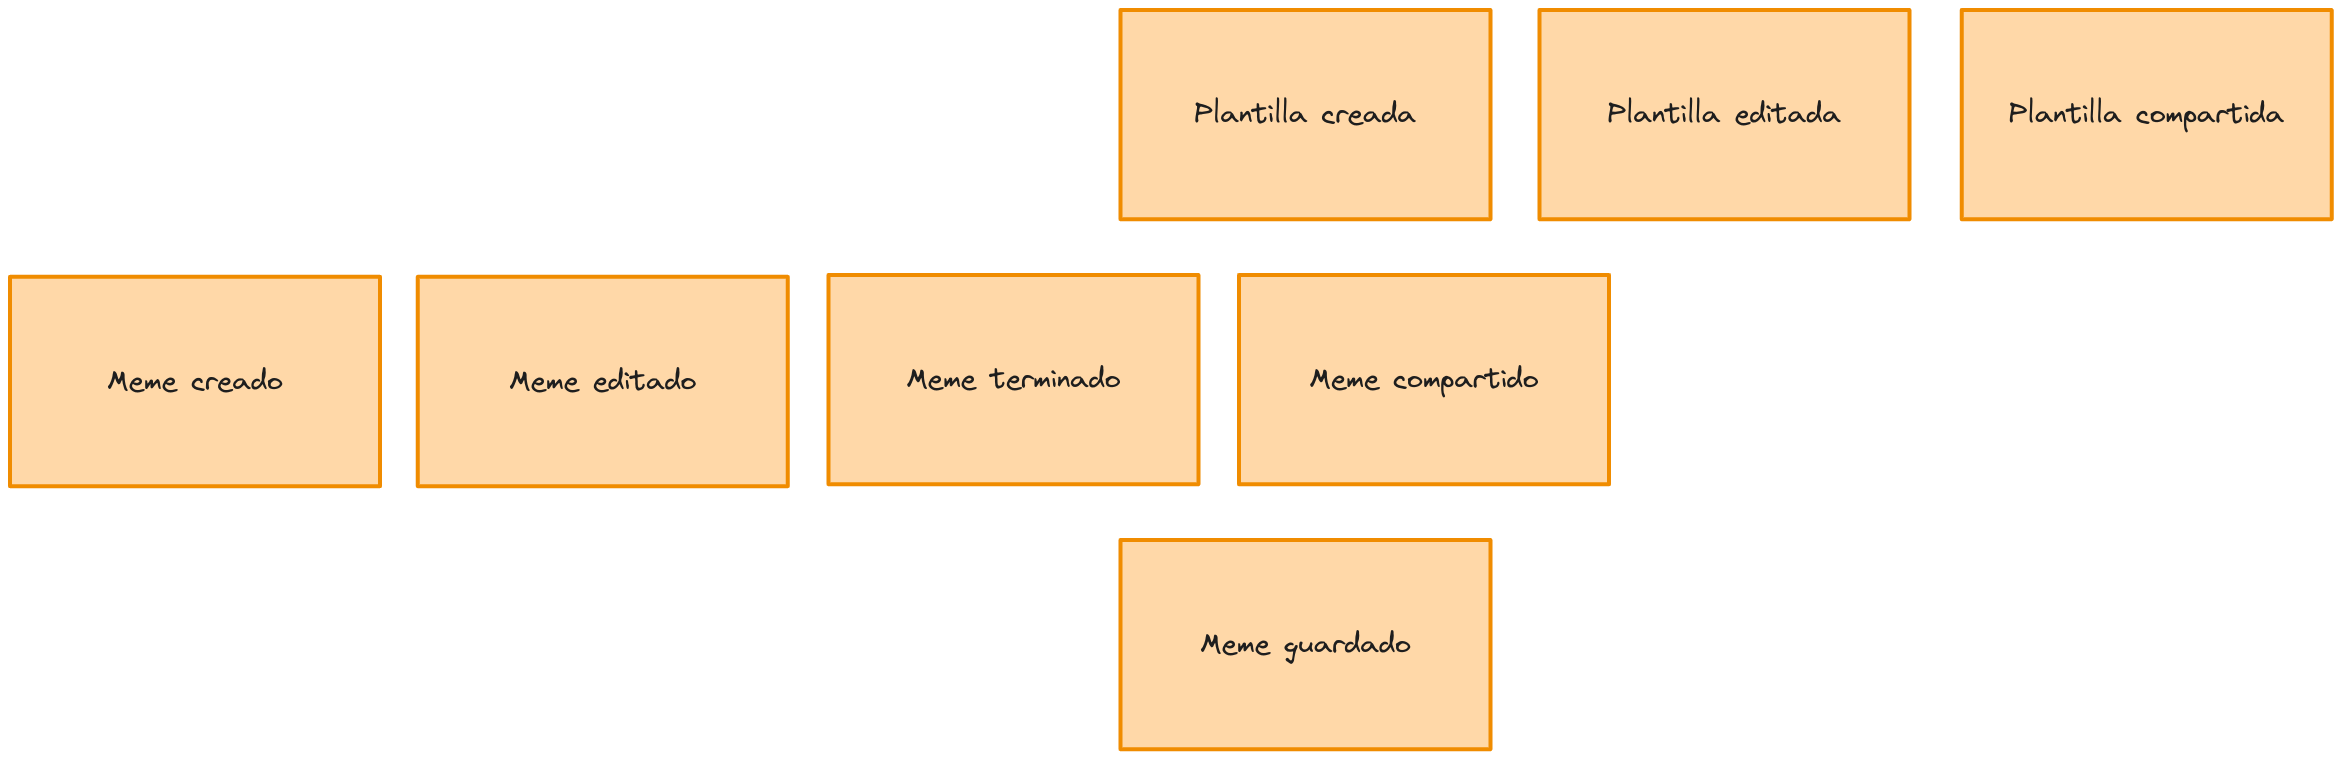
\includegraphics[scale=0.15]{figuras/eventosdominio.png}
\end{figure}

\subsection{Encuentra los límites}

El siguiente paso es encontrar los límites del sistema. Pueden surgir dos tipos de límites:

\begin{itemize}
    \item Límites temporales: los eventos de dominio que a menudo, indican un cambio de un aspecto del sistema son los que especifican estos límites. Si los términos de los eventos cambian, según DDD, acabas de encontrar un contexto delimitado. Se resaltan con una línea azul vertical.
    \item Límites de contexto: estos se encuentran cuando se identifican series de eventos de dominio que utilizan los mismos términos. Se resaltan con una línea azul horizontal dividiendo el diagrama en carriles.
\end{itemize}

\begin{figure}[ht]
    \caption{Límites del sistema.}
    \centering
    \vspace*{0.5cm}
    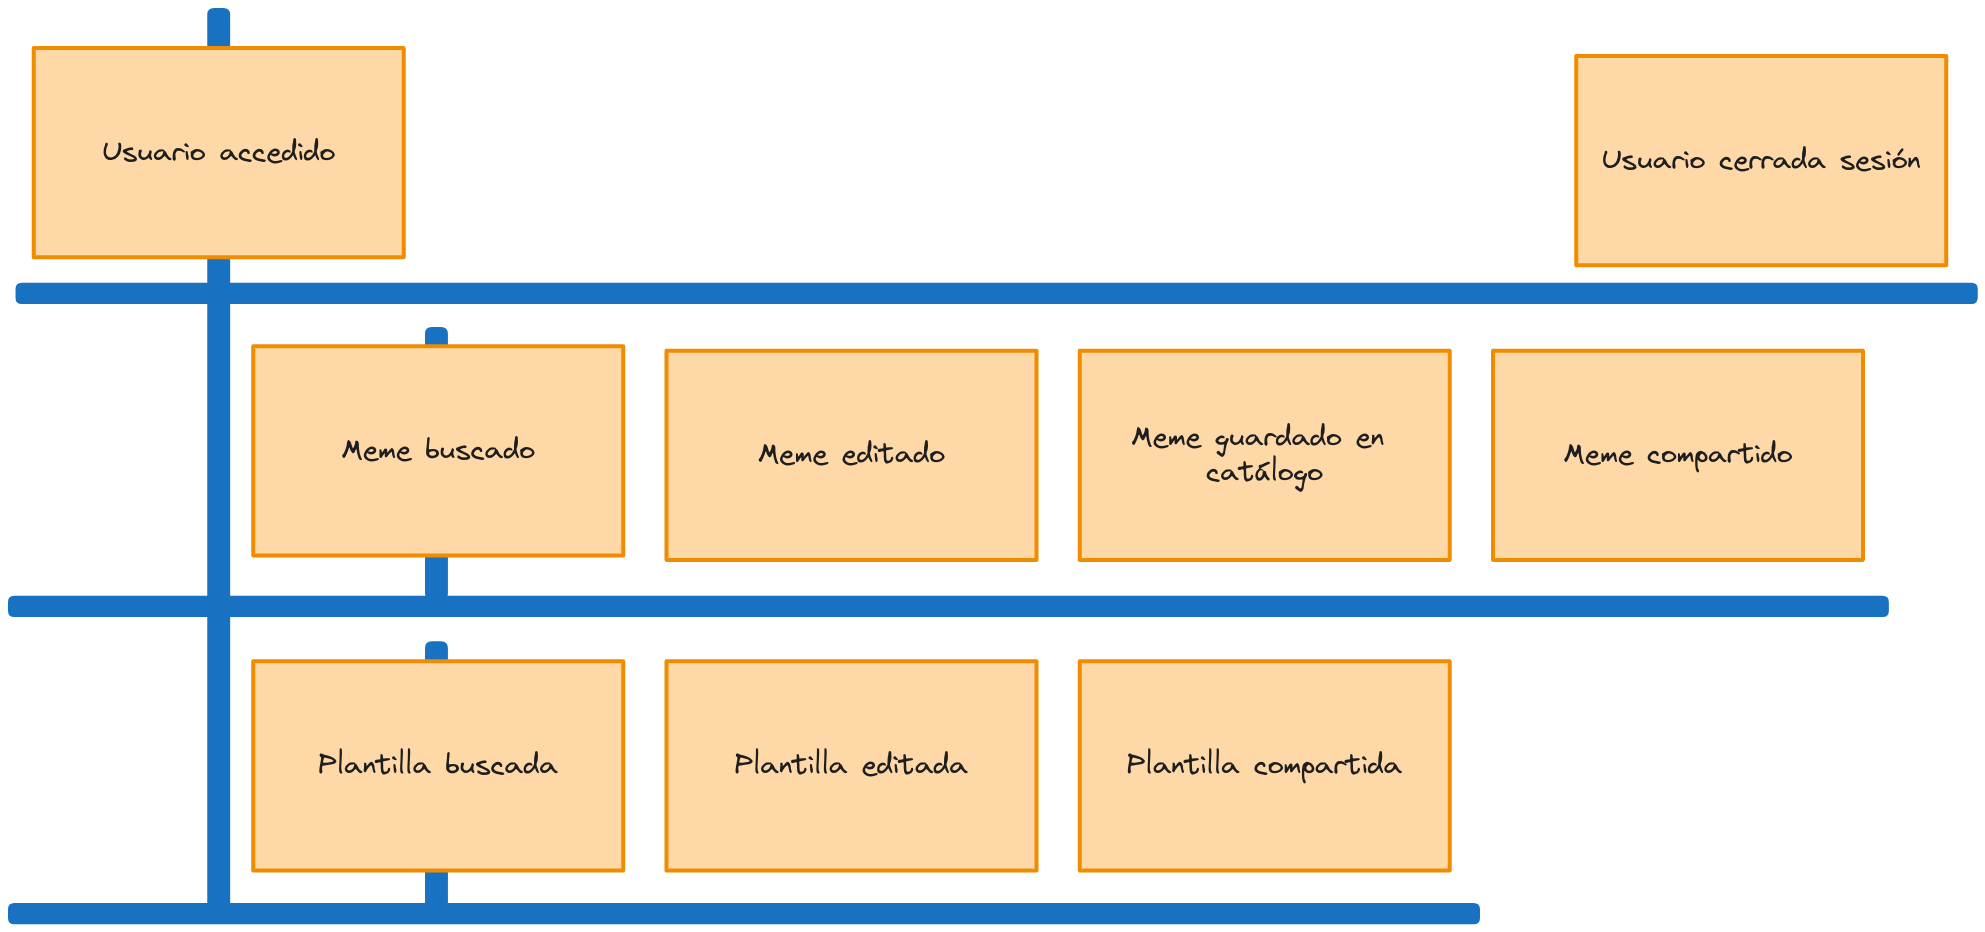
\includegraphics[scale=0.15]{figuras/limites.png}
\end{figure}

\subsection{Localiza los comandos}

Los comandos son el mecanismo más común por el que se crean los eventos de dominio. En este paso el objetivo es identificar las causas cuyos efectos registran los eventos. Estos desencadenantes son los actores, algún sistema externo, una política o algún tipo de marca temporal. El comando que desencadena el evento puede llegar a convertirse más adelante en una llamada a un microservicio o \textit{API}. 



\subsection{\textit{Subdomains} y \textit{bounded contexts}}



